\documentclass[a4paper,10pt,ngerman]{scrartcl}
\usepackage{babel}
\usepackage[T1]{fontenc}
\usepackage[utf8x]{inputenc}
\usepackage[a4paper,margin=2.5cm,footskip=0.5cm]{geometry}
\usepackage{float}
\usepackage{subfigure}
\usepackage{wrapfig}

% Die nächsten drei Felder bitte anpassen:
\newcommand{\Aufgabe}{Aufgabe 4: Fahrradwerkstatt} % Aufgabennummer und Aufgabennamen angeben
\newcommand{\TeilnahmeId}{66432}                  % Teilnahme-ID angeben
\newcommand{\TeamId}{00662}
\newcommand{\Name}{Linus Schumann}             % Name des Bearbeiter / der Bearbeiterin dieser Aufgabe angeben

% Kopf- und Fußzeilen
\usepackage{scrlayer-scrpage, lastpage}
\setkomafont{pageheadfoot}{\large\textrm}
\lohead{\Aufgabe}
\rohead{Teilnahme-ID: \TeilnahmeId, L. Schumann}
\cfoot*{\thepage{}/\pageref{LastPage}}

% Position des Titels
\usepackage{titling}
\setlength{\droptitle}{-1.0cm}

% Für mathematische Befehle und Symbole
\usepackage{amsmath}
\usepackage{amssymb}

% Für Bilder
\usepackage{graphicx}

% Für Algorithmen
\usepackage{algpseudocode}

% Für Quelltext
\usepackage{listings}
\usepackage{color}
\definecolor{mygreen}{rgb}{0,0.6,0}
\definecolor{mygray}{rgb}{0.5,0.5,0.5}
\definecolor{mymauve}{rgb}{0.58,0,0.82}
\lstset{
  keywordstyle=\color{blue},commentstyle=\color{mygreen},
  stringstyle=\color{mymauve},rulecolor=\color{mygray},
  basicstyle=\footnotesize\ttfamily,numberstyle=\tiny\color{mygray},
  captionpos=b, % sets the caption-position to bottom
  keepspaces=true, % keeps spaces in text
  numbers=left, numbersep=5pt, showspaces=false,showstringspaces=true,
  showtabs=false, stepnumber=2, tabsize=2,
  breaklines=true,
  frame=lines,
  framesep=10pt,
  postbreak=\mbox{\textcolor{red}{$\hookrightarrow$}\space}
}

% Anklickbare Links im Dokument
\usepackage{hyperref}
\usepackage{cleveref}
\hypersetup{
    colorlinks,
    citecolor=black,
    filecolor=black,
    linkcolor=black,
    urlcolor=black
}

% Daten für die Titelseite
\title{\textbf{\Huge\Aufgabe}}
\author{\LARGE Teilnahme-ID: \LARGE \TeilnahmeId \\\\
      \LARGE Team-ID: \LARGE \TeamId \\\\
	    \LARGE Bearbeiter/-in dieser Aufgabe: \\ 
	    \LARGE \Name\\\\}
\date{\LARGE\today}

%% ___ Anfang ___ %%
\begin{document}
  \maketitle
  \tableofcontents
  \vspace{4cm}
  %% ___ Lösungsidee ___ %%
  \section{Lösungsidee\label{sec:Loesungsidee}}
    \subsection{Feststellung gegebener Konstanten}
      Als allererstes müssen die Informationen aus der Aufgabenstellung festgestellt werden. Dazu zählen in diesem Fall die Öffnungszeiten. Diese sind jeden Tag identisch und liegen bei 9 bis 17 Uhr. Da die Beispieleingaben alle auf Minuten basieren, macht es Sinn die Öffnungszeiten und alle anderen Zeiten auch in Minuten anzugeben. Daher ergeben sich folgende Konstanten:
      \begin{itemize}
        \item Dauer eines Tages (dt): 1440 min
        \item Dauer der offenen Phase (do): 480 min
        \item Dauer der geschlossenen Phase (dgo): 960 min
        \item Zeitpunkt der Öffnung (to): 540 min
        \item Zeitpunkt des Schließens (tgo): 1020 min
      \end{itemize}
      
    \subsection{Aufgabenteil 1}
      \subsubsection{Abschließen eines Auftrages\label{sec:Loesungsidee:Abschliessen}}
        Jetzt muss überlegt werden, was beim Bearbeiten einer Aufgabe passiert, also wie sich die Gesamtzeit ändert.
        Dazu kann man sich folgenden Ablauf überlegen:
        \begin{enumerate}
          \item Zuerst muss die Dauer des Auftrages so angepasst werden, dass die Öffnungszeiten der Werkstatt berücksichtigt werden. Dies kann wie folgt berechnet werden:
          \begin{equation}
            newDuration = (duration / do)*dt + (duration \mod{do})
          \end{equation}
          Dies bewirkt eigentlich nur, dass für jeden angebrochenen Arbeitstag, die Zeit addiert wird, die das Geschäft geschlossen ist.
          \item Außerdem muss noch falls der Eingangszeitpunkt des Auftrags nach dem aktuellen Zeitpunkt liegt, die Zeit auf den Eingangszeitpunkt gesetzt werden.
          \begin{equation}
            time = startTime
          \end{equation}
          \item Nachdem die Dauer nun an die Arbeitszeiten und der aktuelle Zeitpunkt an den Eingangszeitpunkt angepasst wurde, kann nun die Dauer zur Gesamtzeit addiert werden:
            \begin{equation}
              time = time + newDuration
            \end{equation}
          \item Nach diesem Schritt muss festgestellt werden, ob die Endzeit innerhab der Arbeitszeiten liegt. Dazu muss zuerst die aktuelle Tageszeit berechnet werden:
            \begin{equation}
              dayTime = time \mod{dt}
            \end{equation}
          \item Wenn für diese $dayTime$ $daytime < to$ gilt, liegt der Endzeitpunkt vor der Öffnung und die Dauer der geschlossenen Phase muss noch addiert werden:
            \begin{equation}
              time = time + dgo
            \end{equation}
          \item Dannach ist nur noch möglich, dass der Endzeitpunkt (Erneute Berechnung aus Schritt 3) nach der Schließung der Werkstatt liegt. Er kann nicht mehr am nächsten Tag liegen. Daher muss wenn $dayTime > tgo$ gilt, erneut die Dauer der geschlossenen Phase addiert werden:
            \begin{equation}
              time = time + dgo
            \end{equation}
          \item Am Ende ist es dann möglich die Wartezeit zu berechnen:
            \begin{equation}
              waitingTime = time - startTime
            \end{equation}
        \end{enumerate}
      \subsubsection{Erste Methode\label{sec:Loesungsidee:1}}
        Die erste Methode ist sehr simpel, da einfach nur die Aufträge in der Reihenfolge des Einganges bearbeitet werden. Dafür wird einfach für jeden Auftrag, der in \cref{sec:Loesungsidee:Abschliessen} Ablauf ausgeführt und die resultierende Wartezeit gespeichert. Daraus kann dann die maximale und durchschnittliche Wartezeit berechnet werden.\\
        Die Reihenfolge der Bearbeitung spiegelt das Verhalten einer normalen Queue wieder.
      \subsubsection{Zweite Methode\label{sec:Loesungsidee:2}}
        Die zweite Methode ist im Vergleich zur ersten Methode schon etwas komplexer, da nicht die Reihenfolge des Einganges eingehalten wird, sondern immer der kürzeste Auftrag zuerst bearbeitet wird.\\
        Daher entspricht diese Reihenfolge das Konzept einer Priority Queue.
    \subsection{Aufgabenteil 2\label{sec:Loesungsidee:A2}}
        Das Problem der zweiten Methode (\cref{sec:Loesungsidee:2}) liegt darin, dass eine sehr hohe Maximale Wartezeit entsteht. Dies wird auch durch die Auswertung des ersten Beispiel (\cref{sec:Beispiele:0}) klar deutlich.\\
        Die hohe Wartezeit wird natürlich dadurch erreicht, dass lange Aufträge bei der zweiten Methode sehr oft nach hinten verschoben werden. Allerdings wird dadurch eine sehr niedrige durchschnittliche Wartezeit erreicht.
    \subsection{Aufgabenteil 3}
        Nun muss eine neue Methode erarbeitet werden. Dabei macht es Sinn sich mit den Problemen der 2. Methode auseinander zu setzen. Wie in \cref{sec:Loesungsidee:A2} beschrieben wurde, entsteht die hohe maximale Wartezeit dadurch, dass lange Aufträge sehr oft verschoben werden.\\
        Um dies zum Teil zu verhindert, macht es Sinn eine maximale Anzahl an Verschiebungen nach hinten zu definieren. Diese Maximale Anzahl wird nun mit der Formel $|Warteschlange|*n$ berechnet. $n$ ist eine Konstante für die im Folgenden ein geeigeneter Wert gefunden wird.
        \subsubsection{Bestimmung der Konstante n\label{sec:Loesungsidee:n}}
          Bei der Bestimmung der Konstante $n$ muss zuerst ein Zusammenhang zwischen der maximalen und durchschnittlichen Wartezeit hergestellt werden. Im Folgenden wird dazu eine ''Punktzahl'' mit dieser Formel berechnet:
          \begin{equation}
            score = \max{Wartezeiten} + \overline{Wartezeiten}
          \end{equation}
          In der Menge $Wartezeiten$ ist für jeden Auftrag die Wartezeit gespeichert.\\
          Dann kann für $0\leq n\leq 100$ jeweils die Methode ausgeführt werden und die maximale Punktzahl mit dem zugehörigen Wert für $n$ gespeichert werden.\\
          Wenn dies für jede Beispieldatei ausgeführt wird, kann ein Gesamtdurchschnitt gebildet werden, der fest ins Programm eingebunden werden kann. Eine genauere Auswertung lässt sich in \cref{sec:Umsetzung:Eigene:Auswertung} finden.
  \section{Umsetzung}
    \subsection{Allgemeines}
      Im Folgenden wird die Umsetzung der in \cref{sec:Loesungsidee} beschriebene Lösungsidee, näher erläutert.  Grundsätzlich wurde diese Idee dabei in C++, genauer gesagt in der Datei ''Aufgabe\_4.cpp'' implementiert. Diese Datei befindet sich im Verzeichnis ''./source/''.
      \\\\
      Um das implementierte Programm zu starten kann das Batch Skript ''Aufgabe\_4.bat'' im Verzeichnis ''./executables/'' genutzt werden. Dieses startet das von mir für Windows kompilierte Programm (''Aufgabe\_4.exe''). Für andere Betriebssysteme müsste die Source-Datei erneut auf dem entsprechenden Rechner kompiliert werden.
      \\\\
      Im Verzeichnis ''./beispieleingaben/'' befinden sich alle in dieser Dokumentation aufgeführten Beispiele und im Verzeichnis ''./beispielausgaben/'' befinden sich dementsprechend die gesicherten Ausgaben Letztere werden mit der Datei-Endung ''.out'' gespeichert. Außerdem werden bei jedem Beispiel drei csv-Dateien gesichert, für jede Methode eine. In diesen wird jeweils für jeden Auftrag die Dauer in Verbindung mit der Wartezeit angegeben. Eine Übersicht dieser Daten ist in der Excel-Datei ''Analyse.xlsx'' zu finden. Dabei wurde für jede csv-Datei ein Tabellenblatt mit einem Diagramm erstellt.
    \subsection{Implementation der allgemeinen Funktionen}
      \subsubsection{Daten einlesen}
        Das Einlesen der Daten ist relativ simpel, da einfach die Eingabedatei Zeile für Zeile ausgelesen wird. Die zwei Zahlen die sich dabei in einer Zeile befinden werden dann einfach als ''Pair'' in einer Queue gespeichert. Es macht Sinn eine Queue zu nutzen, da man immer nur den nächsten Auftrag auslesen kann und muss.\\
        Das Einlesen wurde in der Funktion ''readData'' implementiert.
      \subsubsection{Auftrag abschließen} 
        Beim Abschließen eines Auftrages können einfach die mathematischen Schritte aus \cref{sec:Loesungsidee:Abschliessen} verwendet werden. Zusätzlichen wird am Schluss die Wartezeit einem Vektor angefügt und geprüft, ob ein neues Maximum verliegt.\\
        Das Abschließen eines Auftrages wurde in "finishJob" implementiert.
    \subsection{Implementation der ersten Methode}
      Die Implementation der ersten Methode geht einfach nur die Eingabedaten durch. Dabei wird immer der erste Auftrag der Queue bearbeitet und dann gelöscht. Dies passiert solange, bis die Queue leer ist.
    \subsection{Implementation der zweiten Methode}
      Die zweite Methode nutzt eine Priority Queue, um alle aktuell verliegenden Aufträge zu speichern. Diese Priority Queue speichert die Aufträge aufsteigend, sodass am Anfang der Queue immer der kürzeste Auftrag vorliegt. Um die ''Pair-Werte'', die im Input in diesem Format gespeichert wurden: ''{Zeit, Dauer}'', in der Priority Queue nach der Dauer zu sortieren, muss die Reihenfolge innerhalb des Pairs getauscht werden.\\
      Der Ablauf sieht insgesamt so aus, dass solange Eingabedaten verfügar sind, alle bis zum aktuellen Zeitpunkt vorliegenden Aufträge eingelesen werden und dann der kürzeste von diesen bearbeitet wird. Falls zu einem Zeitpunkt noch kein Auftrag vorliegt, wird einfach der nächste gewählt. 
    \subsection{Implementation der eigenen Methode}
      Die eigene Methode funktioniert ähnlich wie die zweite Methode. Es wird nur für jeden Auftrag in der ''Priority Queue'' auch noch die Anzahl an Verschiebungen gespeichert. Beim jeden Abschließen eines Auftrages wird diese Anzahl für jedes Element um 1 erhöht. Um dies umzusetzen kann allerdings keine richtige Priority Queue verwedet werden, da es meines Wissens nicht einfach so möglich ist, über eine Queue zu iterieren. Allerdings kann die Funktionsweise einer Priority Queue auch mit einem Vektor umgesetzt werden, der nach jedem Hinzufügen eines Elementes in den Vektor, sortiert wird. Die Funktion zum Sortieren wurde selbst implementiert und sortiert eigentlich alle Elemente aufsteigend. Allerdings werden Elemente deren Anzahl an Verschiebungen höher ist als die maximale Verschiebung, an den Anfang des Vektors ''geschoben''.
      \subsubsection{Auswertung der Konstante n\label{sec:Umsetzung:Eigene:Auswertung}}
        Wenn man, dass in \cref{sec:Loesungsidee:n} Verfahren anwendet, kommt man insgsamt auf einen Wert von $n=3$. Dieser lässt sich auf jedes Beispiel anwenden und verbessert auch jedes Beispiel im Vergleich zur ersten bzw. zweiten Methode deutlich.
        
  %% ___ Beispiele ___ %%
  \section{Beispiele}
    In diesem Abschnitt befinden sich alle Ausgaben zu allen Beispielen. Außerdem werden zum Beispiel 0 auch noch 3 Diagramme zur Auswertung angegeben.
    \subsection{Beispiel 0\label{sec:Beispiele:0}}
      Das ''erste'' Beispiel wird nun besonders detailiert ausgewertet:\\
      Insgesamt kann man auf Grundlage der Diagramme für die maximale und durchschnittliche Wartezeit feststellen, dass bei der ersten Methode zwar die maximale Wartezeit sehr gering ist, allerdings die durchschnittliche Wartezeit vergleichsweise sehr hoch ist. Die zweite Methode verbessert die durchschnittliche Wartezeit dann enorm, darunter leidet allerdings die maximale Wartezeit deutlich. Schlussendlich verbessert die eigene Methode die durschnittliche Wartezeit im Vergleich zur ersten Methode und die maximale Wartezeit im Vergleich zur zweiten. Daher kann man sagen, dass die eigene Methode beide vorherigen Methoden ''kombiniert'' und damit die beste Methode ist und meinen Erwartungen somit entspricht.
      \begin{figure}[H]
        \centering
        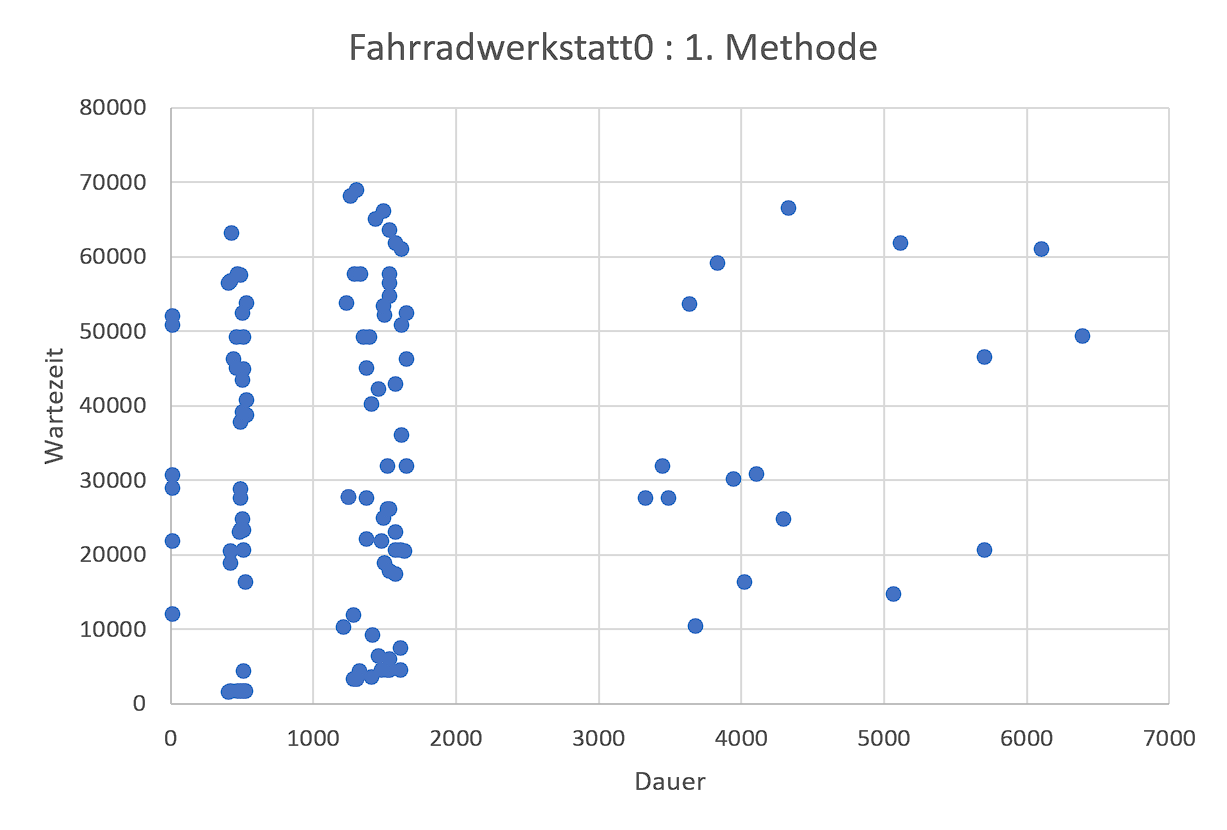
\includegraphics[width=15cm]{../beispielausgaben/fahrradwerkstatt0_sta1.png}
        \caption{Auswertung Beispiel 0: Erste Methode}
        \label{fig:Auswertung01}
      \end{figure}
      \begin{figure}[H]
        \centering
        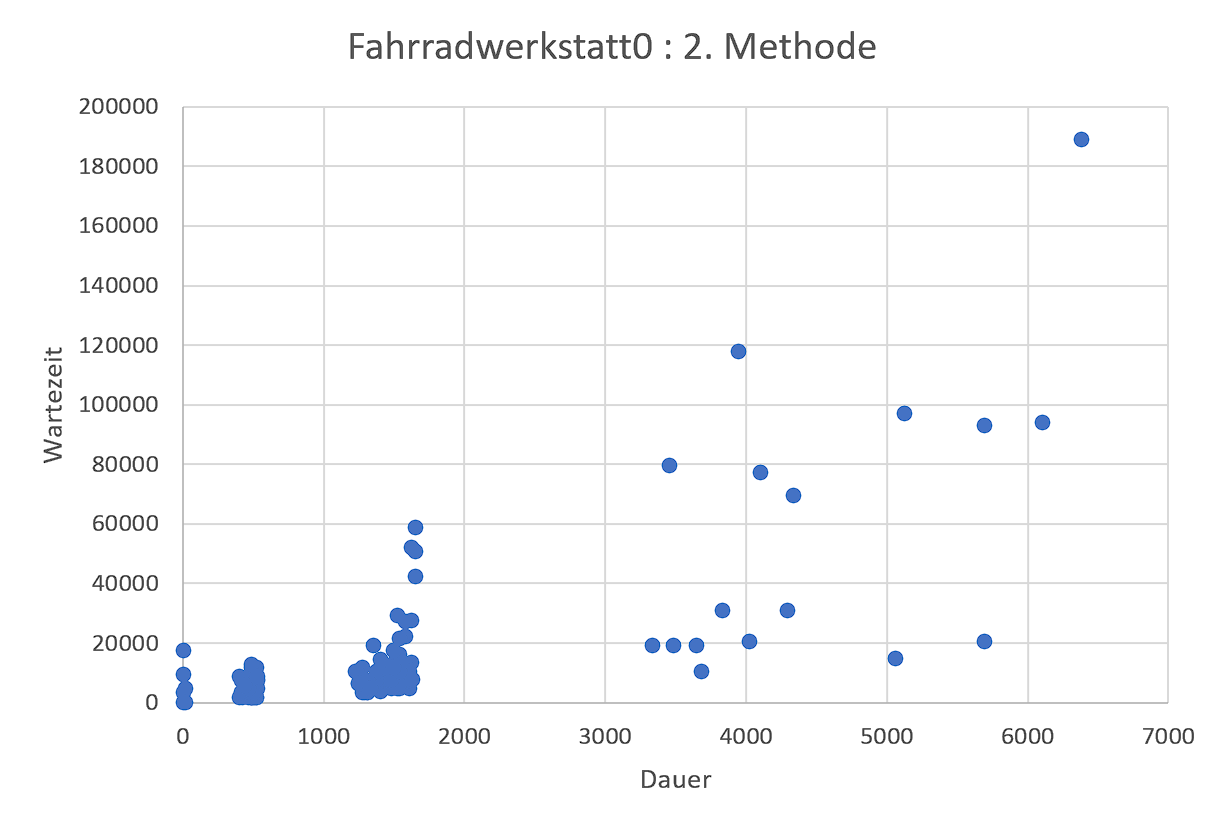
\includegraphics[width=15cm]{../beispielausgaben/fahrradwerkstatt0_sta2.png}
        \caption{Auswertung Beispiel 0: Zweite Methode}
        \label{fig:Auswertung02}
      \end{figure}
      \begin{figure}[H]
        \centering
        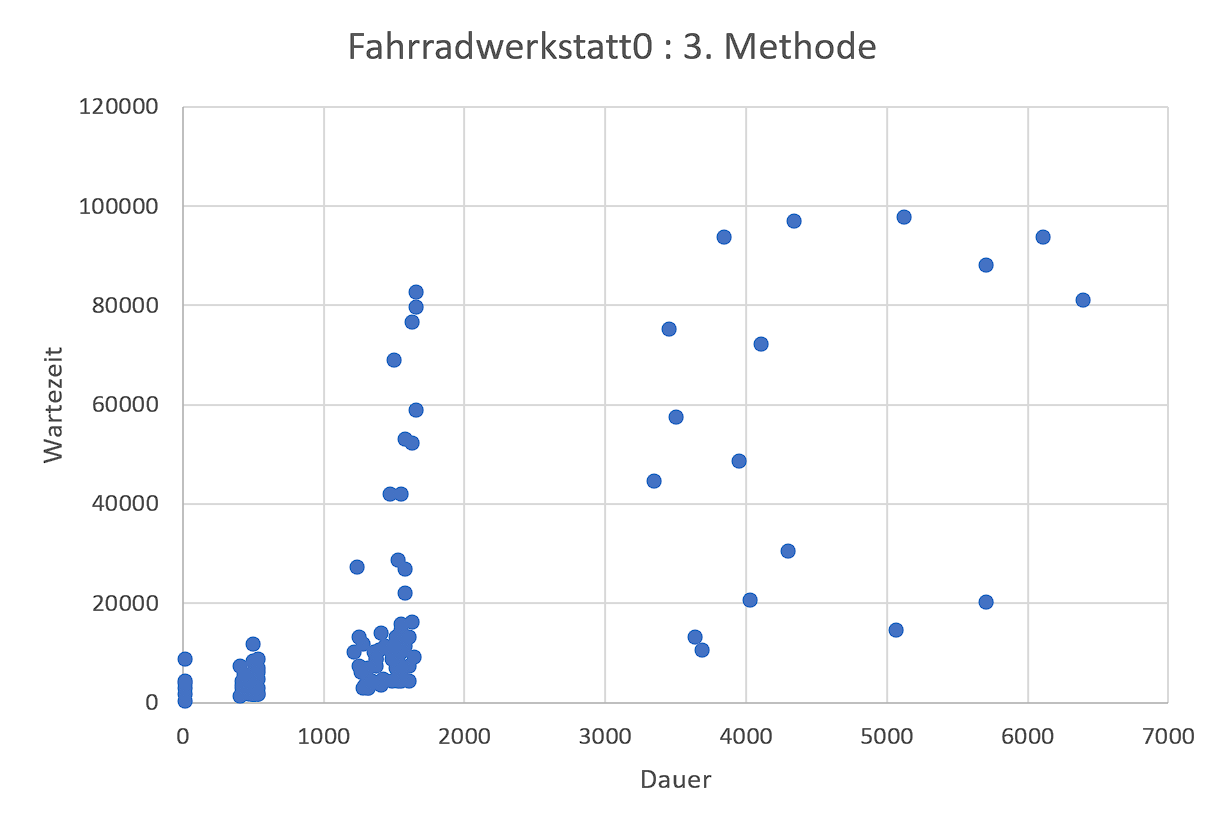
\includegraphics[width=15cm]{../beispielausgaben/fahrradwerkstatt0_sta3.png}
        \caption{Auswertung Beispiel 0: Eigene Methode}
        \label{fig:Auswertung03}
      \end{figure}
    
      \lstinputlisting[caption=Ausgabe Beispiel 0]{../beispielausgaben/fahrradwerkstatt0.out}
    \subsection{Beispiel 1}
      \lstinputlisting[caption=Ausgabe Beispiel 1]{../beispielausgaben/fahrradwerkstatt1.out}
    \subsection{Beispiel 2}
      \lstinputlisting[caption=Ausgabe Beispiel 2]{../beispielausgaben/fahrradwerkstatt2.out}
    \subsection{Beispiel 3}
      \lstinputlisting[caption=Ausgabe Beispiel 3]{../beispielausgaben/fahrradwerkstatt3.out}
    \subsection{Beispiel 4}
      \lstinputlisting[caption=Ausgabe Beispiel 4]{../beispielausgaben/fahrradwerkstatt4.out}
  %% ___ Quellcode ___ %%
  \section{Quellcode}
    \lstinputlisting[language=C++]{../source/Aufgabe_4.cpp}
\end{document}